\documentclass{book}
\usepackage{physics}
\usepackage{graphicx}
\usepackage{caption}
\usepackage{amsmath}
\usepackage[shortlabels]{enumitem}
\usepackage[left=1in,right=1in,top=1in,bottom=1in]{geometry}
\usepackage{bm}
\usepackage{authblk}
\usepackage{empheq}
\usepackage{amsfonts}
\usepackage{esint}
\usepackage[makeroom]{cancel}
\usepackage{dsfont}
\usepackage{centernot}
\usepackage{mathtools}
\usepackage{bigints}
\usepackage{amsthm}
\theoremstyle{definition}
\newtheorem{defn}{Definition}[section]
\newtheorem{prop}{Proposition}[section]
\newtheorem{rmk}{Remark}[section]
\newtheorem{thm}{Theorem}[section]
\newtheorem{exmp}{Example}[section]
\newtheorem{prob}{Problem}[section]
\newtheorem{sln}{Solution}[section]
\newtheorem*{prob*}{Problem}
\newtheorem{exer}{Exercise}[section]
\newtheorem*{exer*}{Exercise}
\newtheorem*{sln*}{Solution}
\usepackage{empheq}
\usepackage{hyperref}
\usepackage{tensor}
\usepackage{xcolor}
\hypersetup{
	colorlinks,
	linkcolor={black!50!black},
	citecolor={blue!50!black},
	urlcolor={blue!80!black}
}



\newcommand{\lambdabar}{{\mkern0.75mu\mathchar '26\mkern -9.75mu\lambda}}



\newcommand*\widefbox[1]{\fbox{\hspace{2em}#1\hspace{2em}}}

\newcommand{\p}{\partial}
\newcommand{\R}{\mathbb{R}}
\newcommand{\C}{\mathbb{C}}
\newcommand{\lag}{\mathcal{L}}
\newcommand{\nn}{\nonumber}
\newcommand{\ham}{\mathcal{H}}
\newcommand{\M}{\mathcal{M}}
\newcommand{\I}{\mathcal{I}}
\newcommand{\K}{\mathcal{K}}
\newcommand{\F}{\mathcal{F}}
\newcommand{\w}{\omega}
\newcommand{\lam}{\lambda}
\newcommand{\al}{\alpha}
\newcommand{\be}{\beta}
\newcommand{\x}{\xi}


\newcommand{\Else}{\text{else}}
\newcommand{\N}{\mathcal{N}}


\newcommand{\sig}{\bm\sigma}
\newcommand{\n}{\mathbf{n}}
\newcommand{\X}{\mathbf{X}}
\newcommand{\s}{\mathbf{S}}

\newcommand{\G}{\mathcal{G}}

\newcommand{\f}[2]{\frac{#1}{#2}}

\newcommand{\ift}{\infty}

\newcommand{\lp}{\left(}
\newcommand{\rp}{\right)}

\newcommand{\lb}{\left[}
\newcommand{\rb}{\right]}

\newcommand{\lc}{\left\{}
\newcommand{\rc}{\right\}}


\newcommand{\V}{\mathbf{V}}
\newcommand{\U}{\mathbf{U}}
\newcommand{\Id}{\mathbb{I}}
\newcommand{\D}{\mathcal{D}}
\newcommand{\Z}{\mathbf{Z}}
\newcommand{\had}{\mathbf{H}}
\newcommand{\Y}{\mathbf{Y}}
%\setcounter{chapter}{-1}


\makeatletter
\renewcommand{\@chapapp}{Chapter}
%\renewcommand\thechapter{$\bf{\ket{\arabic{chapter}}}$}
%\renewcommand\thesection{$\bf{\ket{\arabic{section}}}$}
%\renewcommand\thesubsection{$\bf{\ket{\arabic{subsection}}}$}
%\renewcommand\thesubsubsection{$\bf{\ket{\arabic{subsubsection}}}$}
\makeatother



\usepackage{subfig}
\usepackage{listings}
\captionsetup[lstlisting]{margin=0cm,format=hang,font=small,format=plain,labelfont={bf,up},textfont={it}}
\renewcommand*{\lstlistingname}{Code \textcolor{violet}{\textsl{Mathematica}}}
\definecolor{gris245}{RGB}{245,245,245}
\definecolor{olive}{RGB}{50,140,50}
\definecolor{brun}{RGB}{175,100,80}
\lstset{
	tabsize=4,
	frame=single,
	language=mathematica,
	basicstyle=\scriptsize\ttfamily,
	keywordstyle=\color{black},
	backgroundcolor=\color{gris245},
	commentstyle=\color{gray},
	showstringspaces=false,
	emph={
		r1,
		r2,
		epsilon,epsilon_,
		Newton,Newton_
	},emphstyle={\color{olive}},
	emph={[2]
		L,
		CouleurCourbe,
		PotentielEffectif,
		IdCourbe,
		Courbe
	},emphstyle={[2]\color{blue}},
	emph={[3]r,r_,n,n_},emphstyle={[3]\color{magenta}}
}


\begin{document}
	\begin{titlepage}\centering
		\clearpage
		\title{{\textsc{\textbf{ATOMIC, MOLECULAR, AND OPTICAL PHYSICS}}}\\ \smallskip - A Quick Guide - \\}s
		\author{\bigskip Huan Q. Bui}
		\affil{Massachusetts Institute of Technology}
		\date{\today}
		\maketitle
		\thispagestyle{empty}
	\end{titlepage}

\subsection*{Preface}
\addcontentsline{toc}{subsection}{Preface}

Greetings,\\

This guide is based on 8.421 and 8.422 at MIT, two courses on atomic, molecular, and optical (AMO) physics, taught by Professor Martin Zwierlein between 2022 and 2023. The purpose of this guide is to provide a short summary of the most basic concepts in AMO physics and serve as a reference for PhD qualification exams in this field. This guide may not be treated as a textbook, and the reader may find much more pedagogical resources in the bibliography. Familiarity with undergraduate physics is recommended. \\

\noindent Enjoy! 

\newpage
\tableofcontents
\newpage



%%%%%%%%%%%%%%%%%%%%%%%%%%%%%%%%%%%%%%%%%%%%%%
%%%%%%%%%%%%%%%%%%%%%%%%%%%%%%%%%%%%%%%%%%%%%%



\chapter{Harmonic Oscillators and Resonance}


\section{The Lorentz Oscillator Model}

This model is incredibly powerful and is one of the most fundamental topics to know and understand when learning AMO physics. So let's get started. We will first consider a \textbf{classical harmonic oscillator} first. For non-trivial dynamics, we consider the case where this system is damped and driven. 
\begin{equation}\label{eq:lorentz}
\ddot x + \gamma \dot x + \omega_0^2 x = \f{F_0}{m}\cos(\omega t).
\end{equation}
Here $\gamma,\omega_0,m,F_0$ take their usual meanings. As a review, we shall introduce the general steady-state solution (we typically don't care about transient behavior) and write down the under-damping condition explicitly. To do this, we have to solve the ODE  \eqref{eq:lorentz}. Then, we will answer some questions that will improve our understanding of the model. \\



\noindent \textbf{\underline{What is the general solution?}}  \\


To make the forthcoming algebraic manipulations clearer, let us use complex notations, so that $\cos(\omega t) \to e^{i\omega t}$. Since the problem concerns only the steady-state solution, we shall ignore the transient behavior and consider the following ansatz oscillating at the drive frequency $\omega$:
\begin{align*}
x(t) = A e^{i\omega t } e^{i\phi}
\end{align*}
where $A \in \mathbb{R}$ is the amplitude and $\phi \in \mathbb{R}$ is the phase. Plugging the ansatz into the ODE, we find 
\begin{align*}
x(t) = A e^{i\omega t} e^{i\phi} \implies -A e^{i \omega t + i\phi} \lp \omega^2 -\omega_0^2 - i\gamma \omega \rp = \f{F_0}{m}e^{i\omega t} \implies A = \f{F_0/m}{-\omega^2 + \omega_0^2 + i\gamma \omega} e^{-i\phi}.
\end{align*}
Since $A$ is real, the denominator of $A$ must be a complex number of the form $\abs{A} e^{-i\phi}$ where
\begin{align*}
\abs{A} = \sqrt{{(\omega_0^2 - \omega^2)}^2 + (\gamma \omega)^2}.
\end{align*}
And the phase $\phi$ is\footnote{I should have used $e^{-i\phi}$ so that $\phi$ in this definition would be the phase \textit{lag}... but okay.}
\begin{align*}
\boxed{\phi = -\arctan(\f{\gamma\omega}{\omega_0^2 - \omega^2})}
\end{align*}
With these, we may write
\begin{align*}
\boxed{A = \f{F_0/m}{\sqrt{(\omega_0^2 - \omega^2)^2 + (\gamma \omega)^2}}}
\end{align*}
The oscillator is underdamped, so we want the roots of the associated chacteristic polynomial $\lambda^2 + \gamma \lambda + \omega_0^2 = 0$:
\begin{align*}
\lambda\pm = -\f{\gamma}{2} \pm \f{1}{2}\sqrt{\gamma^2 - 4\omega_0^2}
\end{align*}
to be complex (to get oscillations on top of an exponential decay). As a result, we require that 
\begin{align*}
\gamma^2 < 4\omega_0^2 \iff \boxed{\gamma < 2\omega_0}
\end{align*}
This is the standard underdamping condition. \\


\noindent \textbf{\underline{At which $\omega$ do we get maximal amplitude response?}} \\

Before proceeding, let us introduce two dimensionless quantities $\rho = \omega/\omega_0$ and $f = \gamma/\omega_0$ and rewrite $A$ as 
\begin{align*}
A =  \lp \f{F_0}{m \omega_0^2}\rp \f{1}{\sqrt{(1-\rho^2)^2 + (f\rho)^2}}
\end{align*}
Finding $\omega$ so that $A$ is maximal requires finding $\rho$ for which the denominator of $A$ is minimal:
\begin{align*}
\f{d}{d\rho}\lb (1-\rho^2)^2 + (f\rho)^2 \rb = 2\rho(-2 + f^2 + 2\rho^2).
\end{align*}
Setting the expression above to zero tells us that $\rho$ could be $0$ or $\sqrt{1-f^2/2}$ (we must also verify that $A$ has a global maximum, but I won't go into the details here). Since $f = \gamma/\omega_0 \in (0,2)$ we must consider two cases:
\begin{itemize}
	\item If ${0 < f \leq \sqrt{2}}$ then the solution $\rho = \sqrt{1-f^2/2}$ is real and we have 
	\begin{align*}
	A(0)= \f{F_0}{m\omega_0^2} <  \f{F_0}{m\omega_0^2} \lp \f{2}{f\sqrt{4-f^2}}\rp  = A\lp \sqrt{1-f^2/2}\rp
	\end{align*}
	because $f\sqrt{4-f^2} \leq 2$ for $f\in (0,2)$. We therefore see that $A$ attains its maximum at $$\boxed{\omega = \omega_0 \sqrt{1- \gamma^2/2\omega_0^2}}$$
	
	
	
	\item Otherwise, if ${\sqrt{2} < f < 2}$ then the solution $\rho = \sqrt{1-f^2/2}$ is imaginary and $A$ attains its maximum of $F_0/m\omega_0^2$ at $$\boxed{\omega = 0}$$
\end{itemize}
Contrary to what we might expect, the maximal amplitude is attained \textbf{NOT} at the resonance frequency $\omega_0$. Rather, depending on the ratio $\gamma/\omega_0$, we have different answers. \\



\noindent \textbf{\underline{At which $\omega$ does the phase lag between the response and the drive becomes $\pi/2$?}} \\



The phase \textit{lag} being $\pi/2$ means that $\phi = -\pi/2$, i.e.,
\begin{align*}
\arctan\lp \f{\gamma \omega}{\omega_0^2 - \omega^2} \rp = \f{\pi}{2} \implies \boxed{\omega = \omega_0}
\end{align*}
This means that the resonance condition is better characterized by the $\pi/2$ phase lag of the response relative to the drive, rather than the amplitude attaining its maximal value. \\




\noindent \textbf{\underline{When does the power delivered from the drive to the oscillator become maximal?}} \\

Here, by ``power'' we actually mean the power delivered from the drive averaged over one cycle. The power from the drive is given by $P = dW/dt$ where $dW$ is the work done by the drive over an infinitesimal $dx$ and is thus given by $dW = Fdx$.  Putting everything together we have $P = F(t)x'(t)$. The power delivered from the drive, averaged over one cycle of period $T = 2\pi / \omega$, is therefore
\begin{align*}
\langle P \rangle 
&= \f{\omega}{2\pi}\int_{0}^{2\pi/\omega} F_0 \cos(\omega t) \f{d}{dt} \Re{x(t)} \,dt \\
&= \f{F_0 A \omega}{2\pi}  \int_{0}^{2\pi/\omega} \cos(\omega t)  \f{d}{dt} \cos\lp \omega t + \phi \rp \,dt \\
&= -\f{F_0 A \omega^2}{2\pi}  \int_{0}^{2\pi/\omega} \cos(\omega t) \sin\lp \omega t + \phi \rp \,dt \\
&= -\f{1}{2}F_0 A \omega \sin \phi.
\end{align*} 
Plugging in the expressions for $\phi$ and $\omega$ we find 
\begin{align*}
\boxed{\langle P \rangle = \f{F_0^2 }{2m\gamma}\f{(\gamma\omega)^2}{(\omega_0^2 - \omega^2)^2 + (\gamma \omega)^2}}
\end{align*}
We recognize that $P$ has the form of a Lorentzian (or a Cauchy distribution) with FWHM $\gamma$ which attains the maximum $\langle P \rangle_\text{max} = F_0^2/2m\gamma$ at $\omega = \omega_0$.  \textcolor{blue}{One may also use standard calculus techniques to get this result.} \\



\noindent $\boxed{\textbf{!}}$ It makes sense that the power delivered by the drive to the oscillator, averaged over one cycle, is the same as the power dissipated by the damping, averaged one cycle, since the system is in equilibrium in steady state. This can be verified by repeating the calculation above explicitly, but for the damping force. The work done by drag force is $-m\gamma x'(t)$, from which we find the dissipated power is $P_\text{dis} = Fv = m\gamma v(t)^2$. From here, we have
\begin{align*}
\langle P_\text{dis}\rangle = \f{\omega}{2\pi}m\gamma A^2\int_0^{2\pi/\omega} \lp \f{d}{dt}\cos(\omega t + \phi)\rp^2\,dt = \f{1}{2}m\gamma A^2\omega^2.
\end{align*}
Plugging in the expression for $A$ we find that
\begin{align*}
\langle P_\text{dis}\rangle = \f{F_0^2}{2m\gamma} \f{(\gamma\omega)^2}{(\omega_0^2 - \omega^2)^2 + (\gamma \omega)^2} = \langle P \rangle \,\,\,\checkmark
\end{align*}



\noindent \textbf{\underline{Why does the dissipated power become maximal at that frequency?} } \\


When the drive $F \propto \cos (\omega t)$ is at $\omega = \omega_0$, the position $x(t) \propto \cos(\omega_0 t + \phi)$ of the oscillator has a $-\phi =\pi/2$ phase lag compared to the drive. However, the velocity $x'(t) \propto -\sin(\omega_0 t -\pi/2) = \cos(\omega_0 t)$ is now in phase with the drive. As a result, the drive is always doing positive work, and thus $\langle P \rangle$ is maximal.  \\







\noindent \textbf{\underline{Why does reducing $\gamma$ increase $P$ on resonance?}}\\

In the far off-resonance regime, we may assume that $\abs{\omega_0^2 - \omega^2}\gg \gamma \omega$, so that 
\begin{align*}
\langle P \rangle_\text{far off res.}  \approx   \f{F_0^2}{2m\gamma} \f{(\gamma \omega)^2}{(\omega_0^2 - \omega^2)^2} \propto \gamma,
\end{align*}
so $\langle P \rangle$ varies linearly in $\gamma$ for far off-resonance drive. In the near-resonance regime, we may ignore the term $\omega_0^2 - \omega^2$ in the denominator to find 
\begin{align*}
\langle P \rangle_\text{near res.} \approx \f{F_0}{2m\gamma} \propto \gamma^{-1}.
\end{align*}


As the damping is decreased, the amplitude of the motion increases, thereby increasing the dissipated power on resonance. In the limit of no damping $(\gamma = 0)$, the power dissipated on resonance becomes infinite because the amplitude blows up. The line shape of the response becomes that of a Dirac delta function. \\




\noindent \textbf{\underline{On resonance, what is the steady-state average energy stored and dissipated per cycle?}}\\

Now we have resonant driving, so $\omega = \omega_0$. The steady-state average energy stored in the oscillator is the sum of kinetic and potential energy. 
\begin{align*}
\langle KE\rangle &= \f{\omega_0}{2\pi} \int_0^{2\pi/\omega_0} \f{1}{2}m x'(t)^2\,dt=   \f{F_0^2 }{4m\gamma^2}\\
\langle PE \rangle &= \f{\omega_0}{2\pi}\int_0^{2\pi/\omega_0} \f{1}{2}m \omega_0^2 x(t)^2\,dt  = \f{F_0^2}{4m\gamma^2}
\end{align*}
where we have used $x(t) = (F_0/m\gamma \omega_0) \sin(\omega_0 t)$. From here, the total energy stored in the oscillator is 
\begin{align*}
\boxed{\langle E \rangle = \langle KE \rangle + \langle PE \rangle = \f{F_0^2}{2m\gamma^2}}
\end{align*}
On the other hand, the energy dissipated in one cycle may be calculated by integrating the dissipated power over a cycle $E_\text{lost} = \int P_\text{dis}\,dt$ where $P_\text{dis} = F_\text{damp} v(t)$: 
\begin{align*}
\boxed{E_\text{lost} = \int_0^{2\pi/\omega_0} \gamma m x'(t) x'(t)\,dt = \f{F_0^2 \pi}{m\gamma \omega_0}}
\end{align*}
Take the $2\pi$-adjusted ratio of these two results, we find 
\begin{align*}
2\pi \f{\langle E \rangle}{E_\text{lost}} = \f{\omega_0}{\gamma},
\end{align*}
which is nothing but the \textbf{quality factor} $\boxed{Q = \omega_0 / \gamma}$.\\










\noindent \textbf{\underline{What happens when the mass has charge $q$ and is driven by $F = e\mathcal{E}\cos(\omega t)$?}}\\


This is the \textbf{Lorentz Oscillator Model}. When $\gamma = 0$ (undamped -- we will think about what damping means in this case), the steady-state dipole moment $d(t) = ex(t)$ is given by:
\begin{align*}
d(t) = ex(t) = \f{e^2 E\cos(\omega t)}{\omega_0^2 - \omega^2}.
\end{align*}
This expression is related to a concept called \textbf{oscillator strength} which we will look at later. \\




Even in the absence of other kinds of damping, the motion will be damped because
of what is called \textbf{radiation damping}, $\gamma = \Gamma_{\text{rad}}$. From classical electrodynamics, we know that
any accelerated charge will emit radiation. The total power radiated by an accelerated
electron in the full solid angle of $4\pi$ (see \cite{griffiths2005introduction} for details) is 
\begin{align*}
P = \f{1}{6\pi \epsilon_0 c^3}|\ddot{d}|^2.
\end{align*}



\noindent \textbf{\underline{On resonance, what is the energy lost per orbital cycle?}}\\

Taking the amplitude of $x(t)$ to be $x_0$, the total power radiated in the full solid angle of $4\pi$ is 
\begin{align*}
P = \f{1}{6\pi \epsilon_0 c^3}\abs{\ddot d}^2 = \f{e^2 x_0^2 \omega_0^4 \cos^2(\omega_0 t)}{6 c^3 \pi \epsilon_0}.
\end{align*}
The energy lost per orbital cycle is thus
\begin{align*}
E_\text{lost} = \int_0^{2\pi/\omega_0} P\,dt = \f{e^2 x_0^2 \omega_0^3}{6c^3 \epsilon_0}.
\end{align*}



\noindent \textbf{\underline{From $E_\text{stored}$ and $E_\text{lost}$, what is $\Gamma_\text{rad}$? }}\\

The total energy is calculated in the same manner as before:
\begin{align*}
\langle KE\rangle &= \f{\omega_0}{2\pi} \int_0^{2\pi/\omega_0} \f{1}{2}m x'(t)^2\,dt= \f{1}{4}m \omega_0^2 x_0^2  \\
\langle PE \rangle &= \f{\omega_0}{2\pi}\int_0^{2\pi/\omega_0} \f{1}{2}m \omega_0^2 x(t)^2\,dt  = \f{1}{4}m \omega_0^2 x_0^2 \\
E_\text{stored} &= \langle KE \rangle + \langle PE \rangle = \f{1}{2}m \omega_0^2 x_0^2
\end{align*}
From here, we get
\begin{align*}
Q = 2\pi \f{E_\text{stored}}{E_\text{lost}} = \f{6c^3 m\pi \epsilon_0}{e^2 \omega_0}.
\end{align*}
Since $Q = \omega_0 / \Gamma_{\text{rad}}$, we find
\begin{align*}
\boxed{\Gamma_\text{rad} = \f{\omega_0}{Q} = \f{e^2 \omega_0^2}{6c^3 m \pi \epsilon_0}}
\end{align*} 

\noindent \textbf{\underline{What is $Q$ in terms of the classical radius of the electron and $\lambdabar $ of the emission?}}\\


In terms of the classical radius of the electron
\begin{align*}
r_0 = \f{e^2}{4\pi \epsilon_0 mc^2}, 
\end{align*}
we have
\begin{align*}
Q = \f{3\lambdabar}{2r_0} \quad\quad \text{and}\quad\quad \Gamma_\text{rad} = \f{\omega_0}{Q} = \f{2r_0c}{3\lambdabar^2}
\end{align*}




\noindent \textbf{\underline{Estimate $Q,\Gamma_\text{rad}$ for the Sodium D2 line.}}\\



With $\lambda = 589 $ nm, we have
\begin{align*}
Q &\approx 5.0 \times 10^7 \\
\Gamma_\text{rad} &\approx 2\pi \times 10.2 \text{ MHz}
\end{align*}
which is in remarkable agreement with the experimentally measured natural line width for the D2 line of Na which is $2\pi \times 9.795(11)$ MHz. The calculation is within $\sim 5$\% of the measured value.  





\subsection{The Signal-to-Noise ratio and the quality factor}



Let's look at the expression for the power delivered to the oscillator again:
\begin{align*}
{\langle P \rangle = \f{F_0^2 }{2m\gamma}\f{(\gamma\omega)^2}{(\omega_0^2 - \omega^2)^2 + (\gamma \omega)^2}}
\end{align*}
Near resonance, we may make the following approximation:
\begin{align*}
\omega_0^2 - \omega^2 \approx 2\omega(\omega_0  - \omega),
\end{align*}
so that 
\begin{align*}
\langle P \rangle = \f{F_0^2 }{2m\gamma} \f{1}{1 + \lp \f{\omega - \omega_0}{\gamma/2}\rp ^2}.
\end{align*}
This is a Lorentzian with FWHM $\Delta \omega = \gamma$. The time constant for the decay constant $\gamma$ is simply $\tau = 1/\gamma$. The quality factor is again $Q = \omega_0  / \gamma = \omega_0 / \Delta \omega$. From here, we see that
\begin{align*}
\tau \Delta \omega = 1
\end{align*}
which can be treated as an uncertainty relation, which characterizes \textbf{individual measurements}. This means we can actually find $\omega_0$ to better than $\Delta \omega$ with multiple measurements. To be more precise: In the presence of noise, the frequency precision with which the center can be located, $\delta \omega$, depends on the signal-to-noise ratio via
\begin{align*}
\delta \omega = \f{\Delta \omega}{S/N},
\end{align*}
as a rule of thumb. This means that we can see that with high $S/N$, we can measure $\omega_0$ very precisely. This is what we mean by ``splitting the resonance line.'' Typically, experimenters can split the line by a factor of $10^3$. 


\section{The Quantum Harmonic Oscillator}


Consider a 1D harmonic oscillator of mass $m$ and frequency $\omega$ in a number state $\ket{n}$. \\




\noindent \textbf{\underline{How are the annihilation and creation operators $ a$ and $ a^\dagger$ relate to $ x$ and $ p$?}}\\


Let $a = A  x - i B  p$, where $A,B$ are real scalars, so that $ a^\dagger = A x+ i B  p$. We want the following to hold:
\begin{align*}
\ham = \f{p^2 }{2m} + \f{1}{2}m\omega^2 x^2 = \hbar \omega \lp a^\dagger a + \f{1}{2} \rp
\end{align*}
so we compute
\begin{align*}
\hbar \omega \lp a^\dagger a+ \f{1}{2}\rp = \hbar \omega A^2 x^2 + \hbar \omega B^2 p^2 + \hbar \omega AB + \f{\hbar \omega}{2}
\end{align*}
where we have used $[x,p] = i\hbar $. By setting 
\begin{align*}
A = \sqrt{\f{m\omega}{2\hbar}} \quad\quad B = -\sqrt{\f{1}{2\hbar m\omega}}
\end{align*}
the first equation is satisfied. We therefore conclude that
\begin{align*}
a = \sqrt{\f{m\omega}{2\hbar}} \lp x + \f{i}{m\omega} p \rp \quad\quad a^\dagger = \sqrt{\f{m\omega}{2\hbar}} \lp x - \f{i}{m\omega} p \rp.
\end{align*}
From here, we find 
\begin{align*}
\boxed{x = \sqrt{\f{\hbar}{2 m\omega}}(a^\dagger + a) \quad\quad\text{and}\quad\quad p = i\sqrt{\f{\hbar m\omega }{2}}(a^\dagger - a)}
\end{align*}




\noindent \textbf{\underline{What are the average and rms position and momentum?}}\\


From the results above, we get
\begin{align*}
\bra{n} x \ket{n} = \sqrt{\f{\hbar}{2 m\omega}}\bra{n} a^\dagger + a \ket{n} = 0
\end{align*}
\begin{align*}
\bra{n} p \ket{n} = i\sqrt{\f{\hbar m\omega }{2}}\bra{n} a^\dagger - a \ket{n} = 0
\end{align*}
since both $a^\dagger$ and $a$ respectively send $\ket{n}$ to $\ket{n+1}$ and $\ket{n-1}$ which are orthonormal to $\ket{n}$. Next, 


\begin{align*}
\sqrt{\bra{n}p^2 \ket{n}} &= \sqrt{-\f{\hbar m\omega}{2}\bra{n} (a^\dagger - a)^2 \ket{n} }\\
&= \sqrt{-\f{\hbar m\omega}{2} \bra{n} a^\dagger a^\dagger -a^\dagger a - aa^\dagger + a^2 \ket{n} }\\
&= \sqrt{\hbar m\omega \lp n+ \f{1}{2} \rp}.
\end{align*}

\begin{align*}
\sqrt{\bra{n}x^2 \ket{n}} &= \sqrt{\f{\hbar}{2 m\omega}\bra{n} (a^\dagger + a)^2 \ket{n} }\\
&= \sqrt{\f{\hbar}{2 m\omega}\bra{n} a^\dagger a^\dagger +a^\dagger a + aa^\dagger + a^2 \ket{n} }\\
&= \sqrt{\f{\hbar}{m\omega}\lp n+ \f{1}{2} \rp}.
\end{align*}







\noindent \textbf{\underline{Check the results above using energy and the virial theorem.}}\\



The total energy is 
\begin{align*}
\langle  E\rangle  = \f{\langle p^2\rangle }{2m} + \f{1}{2}m\omega^2 \langle x^2\rangle = \f{1}{2m}\hbar m\omega \lp n+ \f{1}{2} \rp + \f{1}{2}m\omega^2 \f{\hbar}{m\omega}\lp n+ \f{1}{2} \rp  = \hbar \omega\lp n+ \f{1}{2}\rp \,\,\, \checkmark
\end{align*}

Virial theorem: Since $V\propto x^2$, the virial theorem states that $\langle T \rangle  = \langle V \rangle$. From the calculation above, we see that this holds:
\begin{align*}
\langle T \rangle =  \f{1}{2m}\hbar m\omega \lp n+ \f{1}{2} \rp  = \f{1}{2}m\omega^2 \f{\hbar}{m\omega}\lp n+ \f{1}{2} \rp = \langle V \rangle \,\,\, \checkmark
\end{align*}






\noindent \textbf{\underline{What is the rms size and velocity for Na in $\ket{0,0,0}$ with $\omega = 2\pi \times 100$ Hz?}}\\


For a Na atom in the state $\ket{0,0,0}$ of a 3D harmonic potential, we have, by spherical symmetry:
\begin{align*}
\sqrt{\langle r^2\rangle} = \sqrt{3\langle x^2 \rangle } = \sqrt{3(2\cdot 0+1)\f{\hbar}{2m\omega}} = \sqrt{\f{3\hbar}{2m\omega}}.
\end{align*}
With $\omega = 2\pi \times 100 $ Hz and $m_\text{Na} \approx 23 \times 1.66054\times 10^{-27}$ kg, the rms size is
\begin{align*}
\sqrt{\langle r^2\rangle} \approx 2.57 \text{ \textmu m}.
\end{align*}




Similarly, we can find the rms velocity using spherical symmetry:
\begin{align*}
\sqrt{\langle v^2 \rangle} = \f{1}{m}\sqrt{\langle p^2 \rangle} = \f{1}{m}\sqrt{3\langle p_x^2 \rangle} = \f{1}{m}\sqrt{3(2\cdot 0 + 1) \f{\hbar m \omega}{2}} = \sqrt{\f{3\hbar \omega}{2m}}.
\end{align*}
The numerical value for this is
\begin{align*}
\sqrt{\langle v^2 \rangle} \approx 1.61 \text{ mm/s}.
\end{align*}







%%%%%%%%%%%%%%%%%%%%%%%%%%%%%%%%%%%%%%%%%%%%%%
%%%%%%%%%%%%%%%%%%%%%%%%%%%%%%%%%%%%%%%%%%%%%%





\chapter{The Two-Level System}









\section{Magnetic Resonance: Classical Spin in $\mathbf{{B}(t)}$}





\subsection{Classical spin in a magnetic field}

Consider a classical spin in a magnetic field. Let this spin have some angular momentum which we will always write as $\hbar \bm{J}$. The interaction energy is given by 
\begin{align*}
	W = -\bm{\mu} \cdot \cdot \bm{B}.
\end{align*} 
The force acting on the spin is the gradient of this energy function
\begin{align*}
	\bm{F} = -\grad W = \grad (\bm{u}\cdot \bm{B}).
\end{align*}
And the torque on the spin is 
\begin{align*}
	\bm{\tau} = \bm{\mu}\times \bm{B}.
\end{align*}
Here, 
\begin{align*}
	\bm{\mu} = \gamma (\hbar \bm{J})
\end{align*}
stands for the magnetic moment, which is directly related to angular momentum via the \textbf{gyromagnetic ratio $\gamma$}.

Now torque is rate of change of angular momentum, so we have 
\begin{align*}
	\f{d\hbar \bm{J}}{dt} = \bm{\mu}\times \bm{B} \implies \boxed{\f{d\bm{J}}{dt} = \gamma \bm{J}\times \bm{B} = -\gamma \bm{B}\times \bm{J}}
\end{align*}
This says that the motion of $\bm{J}$ is pure precession about $\bm{B}$, where $\bm{J}$ has constant magnitude and tipping angle $\theta$ relative to $\bm{B}$. The rate of precession is determined by the magnetic field strength $B$ and the gyromagnetic ratio $\gamma$:
\begin{align*}
	\Omega_L = -\gamma B.
\end{align*}
This rate of precession is called the \textbf{Larmor frequency}.\\



\noindent \underline{\textbf{Example:}} Consider an electron traveling with velocity $v$ in a circular loop of radius $r$ and area $A = \pi r^2$. We may consider a current $I = dq/dt = e v/2\pi r$ associated with this motion and find the magnetic moment to be $\bm{\mu} = I A \hat{\bm{z}}$. It is easy to see that 
\begin{align*}
	\bm{\mu} = I A \hat{\bm{z}} = \f{evr}{2} \hat{\bm{z}} = \f{e}{2m} mvr \hat{\bm{z}} = \lp \f{e\hbar}{2m} \rp \lp \f{L}{\hbar} \rp \hat{\bm{z}}
\end{align*}
Here, the quantity $e\hbar / 2m$ is the famous \textbf{Bohr magneton}, $\mu_B$. It is important to remember that for electrons, $\gamma_e \approx -2\mu_B$, whereas for classical charge distributions with $L = \hbar$, $\gamma \approx \mu_B$. This discrepancy has to do with the fact that electrons have two spin states, whereas the latter each has 3 spins states, spaced by $\mu_B$.





\subsection{Rotating coordinate transformation}


Consider a vector $\bm{A}$ rotating with angular velocity $\bm{\Omega}$. The equation of motion is 
\begin{align*}
	\f{d}{dt} \bm{A} = \bm{\Omega} \times \bm{A}.
\end{align*}



Now suppose we have a vector  $\bm{A}$ and we go to a system rotating at angular velocity $\bm{\Omega}$ then 
\begin{align*}
	{\lp \f{d\bm{A}}{dt} \rp_\text{inertial} = \lp \f{d\bm{A}}{dt} \rp_\text{rotating} + \bm{\Omega}\times \bm{A}}
\end{align*}
So to go from an inertial to rotating frame we do the following:
\begin{align*}
	\boxed{\lp \f{d}{dt}\cdot \rp_r = \lp \f{d}{dt}\cdot \rp_i - \bm{\Omega}\times \cdot}
\end{align*}
Now consider the vector $\bm{J}$ like before:
\begin{align*}
	\lp \f{d\bm{J}}{dt} \rp_\text{rot}  =  \lp \f{d\bm{J}}{dt} \rp_\text{inertial} - \bm{\Omega}\times \bm{J} = \gamma \bm{B}\times \bm{J} - \bm{\Omega}\times \bm{J} = \gamma \bm{J}\times (\bm{B} + \bm{\Omega}/\gamma)
\end{align*}
If we let 
\begin{align*}
	\bm{B}_\text{eff} = \bm{B} + \bm{\Omega}/\gamma
\end{align*}
then we have a new equation of motion in the frame rotating at $\bm{\Omega}$:
\begin{align*}
	\lp \f{d\bm{J}}{dt} \rp_\text{rot} = \gamma \bm{J} \times \bm{B}_\text{eff}.
\end{align*}
We see that in the rotating frame, $\bm{J}$ precesses about this new effective magnetic field. Notice that $\bm{J}$ is constant in this frame exactly when $\bm{\Omega} = -\gamma \bm{B}$, which is what we saw before.




\subsection{Larmor's Theorem}

The result above is Larmor's Theorem, which states that the effect of a magnetic field on a free charge can be eliminated by a suitable rotating coordinate transformation. \\


Consider a charged particle in a magnetic field $\bm{B}$, under the influence of some applied force $\bm{F}_0$. The total force on the particle is 
\begin{align*}
	\bm{F} = \bm{F}_0 + q\bm{v}\times \bm{B}.
\end{align*}
In a frame rotating at $\bm{\Omega}$, the force is 
\begin{align*}
\bm{F}_{\text{rot}} &= \bm{F} - 2m(\bm{\Omega}\times \bm{v}_\text{rot}) - m\bm{\Omega} \times (\bm{\Omega}\times \bm{r})\\
&= \bm{F}_0 + q\bm{v}\times \bm{B} + 2m\bm{v}\times \bm{\Omega} - m\bm{\Omega}\times (\bm{\Omega}\times \bm{r}).
\end{align*}
from classical mechanics and substitution. Notice that if we take $\bm{B} = B\hat{\bm{z}}$ and choose 
\begin{align*}
	\bm{\Omega} = -(q/2m)\bm{B}
\end{align*}
then 
\begin{align*}
	\bm{F}_\text{rot} = \bm{F}_0 - m\lp \f{qB}{2m} \rp^2 \hat{\bm{z}} \times (\hat{\bm{z}} \times \bm{r}).
\end{align*}
Typically the $B^2$ term is small, so we may drop it to obtain 
\begin{align*}
	\bm{F}_\text{rot} = \bm{F}_0.
\end{align*}
We see that for the case of a charged particle in a magnetic field $B_0$, by going to a rotating frame with $\Omega = qB/2m $, we are able to eliminate the effect of $B_0$.





\subsection{Motion in a rotating magnetic field}

So far we have considered static magnetic fields and transformed between inertial and rotating frames whose angular velocity is dependent on the field strength and the gyromagnetic ratio (remember that $\Omega = \gamma B$). Now, we will consider what happens when the magnetic field itself rotates. \\


The setup is as follows. Consider a magnetic moment $\bm{\mu}$ precessing about a static field $\bm{B}_0 = B_0 \hat{\bm{z}}$. The rate of precession, a.k.a. the Larmor frequency, is $\omega_0 = \gamma B_0$. The motion of the moment is given by 
\begin{align*}
	\mu_z = \mu\cos\theta, \quad \mu_x = \mu\sin\theta \cos\omega_0t, \quad \mu_y = -\mu\sin\theta \sin\omega_0 t.
\end{align*}


Now we introduce an additional magnetic field $\bm{B}_1$ in the $xy$-plane which rotates at a constant angular frequency $\omega$. We consider two cases. \\



\noindent \textbf{Exact resonance:} In this case, $\omega = \omega_0 = \gamma B_0$. In this case, the full magnetic field is 
\begin{align*}
	\bm{B}(t) = B_1(\cos\omega_0 t \,\, \hat{\bm{x}} -\sin\omega_0 t \,\, \hat{\bm{y}}) + B_0 \hat{\bm{z}}
\end{align*}


What is the motion of $\bm{\mu}$? To do this, we go the frame rotating with $\bm{B}_1$. In this frame, the $z$-axis is the same as the inertial frame, and the $xy$-plane rotates with $\bm{B}_1$. It is easy to see that in this frame, the rotating magnetic field is constant. The effective magnetic field in this frame is thus
\begin{align*}
	\bm{B}_\text{eff}(t) 
	&= \bm{B}(t) - (\omega_0/\gamma) \hat{\bm{z}}\\
	&= B_1(\cos\omega_0 t \,\, \hat{\bm{x}} -\sin\omega_0 t \,\, \hat{\bm{y}}) + (B_0 - \omega_0/\gamma) \hat{\bm{z}}\\
	&= B_1 \hat{\bm{x}}'  + (B_0 - \omega_0/\gamma) \hat{\bm{z}}\\
	&= B_1 \hat{\bm{x}}'.
\end{align*}

Notice that all time dependence is removed. In the rotating frame, the magnetic field is static in the $x$-axis and has value $B_1$, the strength of the rotating magnetic field. The motion of the moment in the rotating frame is then very simple: the problem is reduced to that for a moment in a static field. It is clear that the moment, in this rotating frame, precesses around the $B_1 \hat{\bm{x}'}$ field at angular velocity:
\begin{align*}
	\omega_R = \gamma B_1.
\end{align*}
This is called the \textbf{Rabi frequency}. Remember the difference between Larmor and Rabi frequency! If the moment initially points along the positive $z$-axis, then after $t = \pi/\omega_R$, the moment points the negative $z$-axis: it has completely turned over. 

\begin{figure*}[!htb]
	\centering
	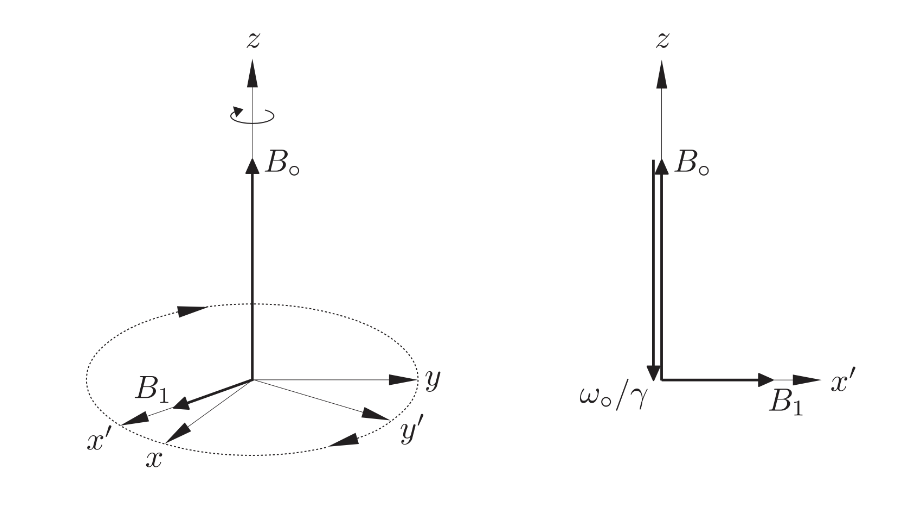
\includegraphics[width=0.7\textwidth]{figures/rotatingB.png}
\end{figure*}


In the inertial frame, the motion of the moment is a combination of precession around the $\hat{\bm{x}}'$ axis (at Rabi frequency $\omega_R = \gamma B_1$) and the rotation of $\hat{\bm{x}}'$ around the $z$-axis (at rate $\omega = \gamma B_0$). 


 




\noindent \textbf{Off-resonant behavior:}  In this case, the rotating magnetic field rotates at a rate $\omega \neq \omega_0 = \gamma B_0$, and therefore:
\begin{align*}
	\bm{B}_\text{eff}(t) = B_1 \hat{\bm{x}}' + (B_0 - \omega_0/\gamma) \hat{\bm{z}}.
\end{align*}

There is still no time dependence, so the effective magnetic field is still static. However, this field makes an angle $\theta$ with the $z$-axis. Since the field is static, we also know that the moment (in the rotating frame) precesses about it, at a rate given by the gyromagnetic ratio $\gamma$ multiplied by the strength of the effective field: 
\begin{align*}
	\boxed{\Omega_R = \gamma B_\text{eff} = \gamma \sqrt{(B_0 - \omega/\gamma)^2 + B_1^2} = \sqrt{(\omega_0 - \omega)^2 + \omega_R^2}}
\end{align*}
This quantity is called the \textbf{generalized Rabi frequency}.\\


Suppose the moment points along the positive $z$-axis like before. What, then, is its motion? The motion of its $x$-component is more complicated and less relevant so we will ignore that. Motivated by quantum mechanics, we will only care about its $z$-component. Finding $\mu_z(t)$ is a simple geometry problem. The answer is 
\begin{align*}
	\boxed{\mu_z(t) = \mu\lb 1 - 2\f{\omega_R^2}{\Omega_R^2}\sin^2 \f{\Omega_R t}{2} \rb}
\end{align*}
Notice that $\mu_z(t)$ never completely flips sign unless $\omega = \omega_0$. It turns out that the quantum mechanical result (which we will soon find) is identical. 




\subsection{Rapid Adiabatic Passage: Landau-Zener Crossing}

Rapid adiabatic passage is a technique for spin-flipping a population by sweeping through resonance. This ``sweeping through resonance'' is achieved when the frequency of the oscillating field ($\omega$) or the transition frequency ($\omega_0$) is \textit{slowly} varied. \\


The problem is essentially solved in view of the last two subsections, so here we present a qualitative solution to strengthen our intuition. Consider the setup as before, with the exception that the rotating field $\bm{B}_1$ initially rotates slowly and far from resonance $\omega \ll \omega_0 = \gamma B_0$. In the rotating frame, the effective magnetic field $\bm{B}_\text{eff}$ is approximately the field in the inertial frame, but without rotation. The magnetic moment precesses about $\bm{B}_\text{eff}$, making a tight angle with it (Here we assume that the moment is initially aligned with the $z$-axis). \\

Now, if we slowly sweep $\omega$ through resonance ($\omega_0$), the magnetic moment will continue to precess tightly around $\bm{B}_\text{eff}$ and will follow it adiabatically.  Eventually, when $\omega \gg \omega_0  = \gamma B_0$, the magnetic moment will be inverted. 


\begin{figure*}[!htb]
	\centering
	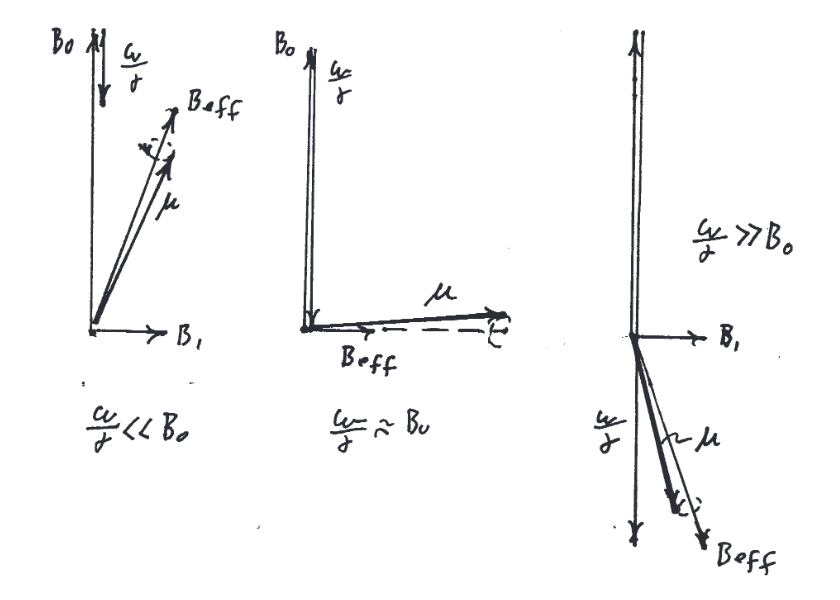
\includegraphics[width=0.75\textwidth]{figures/LZ_following}
\end{figure*}


How slow is \textit{slow}? In order for this adiabatic following to happen, we must require that within one precession period $2\pi/\Omega_R$, the angle that $\bm{B}_\text{eff}$ makes with the $z$-axis must not have advanced by more than a few degrees (Remember that in the expression $B_\text{eff} = B_0 - \omega/\gamma$, the rotation rate $\omega$ is changing.) So, we must have that
\begin{align*}
	\Delta \theta = \dot{\theta} \cdot \Delta t = \dot \theta \f{2\pi}{\Omega_R}  \ll 2\pi \implies \dot \theta \ll \Omega_R,
\end{align*}
i.e., the generalized Rabi frequency $\Omega_R$ must be large compared to the rate at which $\bm{B}_\text{eff}$ is changing direction. Since $B_\text{eff}(t)= B_0 - \omega(t)/\gamma$, and the fact that this requirement is most severe near exact resonance where $\omega = \omega_0 \implies \theta = \pi/2$. So we want:
\begin{align*}
	\f{1}{\gamma B_1} \f{d\omega}{dt} \ll \omega_R.
\end{align*}
But since $\omega_R = \gamma B_1$, the condition is 
\begin{align*}
	\boxed{\dot{\omega} \ll \omega_R^2}
\end{align*}
To summarize, in order for rapid adiabatic passage to occur, we want to slowly sweep from far off-resonance through resonance. To do this, we have to compare $\omega$ to $\omega_0$ and $\dot \omega$ to $\omega_R^2$ and make sure the conditions above hold. \\




A few things to notice. First, the argument above applies for the case where we sweep $\omega$ from above ($\gg \omega_0$) to below ($\ll \omega_0$). Second, rapid adiabatic passage is generally \textit{slower} than a spin-flip using an on-resonance $\pi$-pulse. This is because $\dot \omega$ must be small compared to $\omega_R^2$ (and thus $\omega_R$). 


\subsection{Adiabatic Following in a Magnetic Trap}


As an aside, LZ-crossing explains atom-losses in magneto-optical traps. This happens when an atom traverses through the zero-field region in the MOT. As it does, the rate of change of the field becomes infinitely large, and the atoms fails to follow the field adiabatically and undergoes a spin flip which removes it from the trap. The size of this region is dictated by the speed of the atom $v$ and the gyromagnetic ratio $\gamma$, and the field gradient $B'$:
\begin{align*}
	r = \sqrt{\f{v}{\gamma B'}}.
\end{align*}
This region is also called the \textbf{Majorana hole}.









\section{Resonance of a Quantized Spin}




\subsection{Expectation value of magnetic moment behaves classically}


Now we treat this problem quantum mechanically. First, we will show that the expectation value of magnetic moment behaves classically. 



\subsection{The Rabi Problem}

take this section from the HW


\subsection{Rapid Adiabatic Passage (Landau-Zener) in a QM treatment}


\subsection{Adiabatic Passage}



\section{Density Matrix Formalism}











\section{Atomic Units}





%%%%%%%%%%%%%%%%%%%%%%%%%%%%%%%%%%%%%%%%%%%%%%
%%%%%%%%%%%%%%%%%%%%%%%%%%%%%%%%%%%%%%%%%%%%%%


\chapter{The Basics of an Atom}






%%%%%%%%%%%%%%%%%%%%%%%%%%%%%%%%%%%%%%%%%%%%%%
%%%%%%%%%%%%%%%%%%%%%%%%%%%%%%%%%%%%%%%%%%%%%%


\chapter{Fine Structure and Lamb Shift}














%%%%%%%%%%%%%%%%%%%%%%%%%%%%%%%%%%%%%%%%%%%%%%
%%%%%%%%%%%%%%%%%%%%%%%%%%%%%%%%%%%%%%%%%%%%%%


\chapter{Effects of the Nucleus on Atomic Structure}










%%%%%%%%%%%%%%%%%%%%%%%%%%%%%%%%%%%%%%%%%%%%%%
%%%%%%%%%%%%%%%%%%%%%%%%%%%%%%%%%%%%%%%%%%%%%%




\chapter{Atoms in Magnetic Fields}









%%%%%%%%%%%%%%%%%%%%%%%%%%%%%%%%%%%%%%%%%%%%%%
%%%%%%%%%%%%%%%%%%%%%%%%%%%%%%%%%%%%%%%%%%%%%%



\chapter{Atoms in Electric Fields}





%%%%%%%%%%%%%%%%%%%%%%%%%%%%%%%%%%%%%%%%%%%%%%
%%%%%%%%%%%%%%%%%%%%%%%%%%%%%%%%%%%%%%%%%%%%%%





\chapter{Atoms in Electromagnetic Fields}











%%%%%%%%%%%%%%%%%%%%%%%%%%%%%%%%%%%%%%%%%%%%%%
%%%%%%%%%%%%%%%%%%%%%%%%%%%%%%%%%%%%%%%%%%%%%%



\chapter{Resonance Line Shapes}






%%%%%%%%%%%%%%%%%%%%%%%%%%%%%%%%%%%%%%%%%%%%%%
%%%%%%%%%%%%%%%%%%%%%%%%%%%%%%%%%%%%%%%%%%%%%%




\chapter{Miscellaneous}

This chapter is dedicated to miscellaneous topics that are typically not ``standard'' in an AMO course. These include experimental techniques, advanced processes, and so on. The topics covered here are added in no particular order. The reader may find the \texttt{Search} function useful when browsing through this chapter. 

\section{Atom interferometry and related topics}

\section{Avoided crossing}

\section{Feshbach resonance}











\bibliographystyle{abbrv} 
\bibliography{HuanBui_AMO_refs}% Produces the bibliography via BibTeX.




	
	
\end{document}